\pdfoutput=1
\documentclass[preview]{standalone}

\usepackage[utf8]{inputenc}
\usepackage{lmodern}
\usepackage[T1]{fontenc}

\usepackage{verbatim}
\usepackage{graphicx}
	\DeclareGraphicsRule{*}{mps}{*}{}
\usepackage{xcolor}

\usepackage{tikz}
	\usetikzlibrary{calc}
	\usetikzlibrary{arrows}
	\usetikzlibrary{backgrounds}
	\usetikzlibrary{decorations.pathmorphing}
	\usetikzlibrary{shapes.geometric}
	\tikzset{>=latex'}

\usepackage{amsmath}
\usepackage{amssymb}
\usepackage{dsfont}
\usepackage{nicefrac}
\usepackage{mathrsfs}
\usepackage[Euler]{upgreek}
\usepackage[nointegrals]{wasysym}
\usepackage{booktabs}
\usepackage{float}

\begin{document}

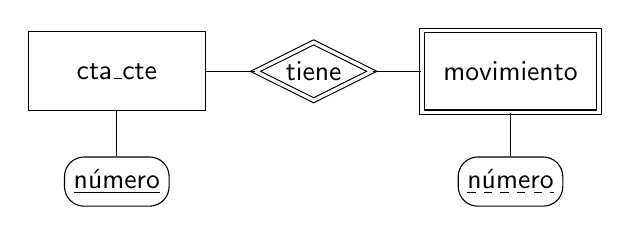
\begin{tikzpicture}[font=\sffamily]
	\node[draw,minimum width=2.25cm,inner ysep=4mm] (cta cte) at (0,0) {cta\_cte};
	\node[draw,double,double distance=1.2pt,minimum width=2.25cm,inner ysep=4mm] (movimiento) at (5,0) {movimiento};
	\node[draw,shape aspect=2,diamond,double,double distance=1.2pt,inner sep=0.5mm] (tiene) at (2.5,0) {tiene};
	\draw (cta cte) -- (tiene) -- (movimiento);
	\node[draw,rounded corners=2.5mm,minimum height=6.25mm] (num) at (0,-1.4) {$\underline{\text{número}}$};
	\draw (cta cte)--(num);
	\node[draw,rounded corners=2.5mm,minimum height=6.25mm] (cod) at (5,-1.4) {número\makebox[0pt][c]{\phantom{$\underline{\text{número}}$}}};
	\draw (movimiento)--(cod);
	\draw[dashed] (4.45,-1.535)--(5.55,-1.535);
\end{tikzpicture}

\end{document}
